% !TeX program = lualatex
% !BIB program = biber
% Lualatex is important to render TTF fonts; with pdflatex it's just the regular one
% ratio 16:9 -- https://tex.stackexchange.com/questions/14336/

% compile two versions, inspired by https://tex.stackexchange.com/a/1501
% use the script "compile-pdf.sh"
\newif\ifhandout
% if flags.tex does not exist, create an empty file to be able to compile in TeXstudio
\input{flags}

\ifhandout
\documentclass[12pt,aspectratio=169,handout]{beamer}
\else
\documentclass[12pt,aspectratio=169]{beamer}
\fi


\input{../include/header-include.tex}

% for redacting text
\usepackage{censor}

\newcommand{\mybox}[1]{\fcolorbox{black!30}{gray!10}{\scriptsize #1}}



\title{Privacy-Preserving Natural Language Processing}
\subtitle{Lecture 3 -- Introduction to Differential Privacy}
\date{May 7, 2026}
\author{Prof.\ Dr.\ Ivan Habernal}
\institute{
\texttt{www.trusthlt.org} \\
Trustworthy Human Language Technologies Group (TrustHLT) \\
Ruhr University Bochum \& Research Center Trustworthy Data Science and Security}



\begin{document}

\maketitle


\section{Intro}

\begin{frame}{Overview}

First lecture: privacy definitions, arbitrary hard choices

Second lectures: still arbitrary choice in anonymization, but GDPR notion of possibility of deidentification

Today: towards probabilistic approach to privacy


%\begin{tikzpicture}[overlay, remember picture]
%\node at (current page.north east)[ref] {
%\fullcite{Voigt.Bussche.2017} \par};
%\end{tikzpicture}
\end{frame}


\section{Differential privacy basics}



\begin{frame}{Precursors of differential privacy}

"Let us begin with a short story. Envision a database of a hospital containing the medical history of some population. On one hand, the hospital would like to advance medical research which is based (among other things) on statistics of the information in the database. On the other hand, the hospital is obliged to keep the privacy of its patients, i.e. leak no medical information that could be related to a specific patient. The hospital needs an access mechanism to the database that allows certain ‘statistical’ queries to be answered, as long as they do not violate the privacy of any single patient."


\begin{tikzpicture}[overlay, remember picture]
\node at (current page.north east)[ref] {
\fullcite{dinurRevealingInformationPreserving2003} \par};
\end{tikzpicture}
\end{frame}



\begin{frame}{Precursors of differential privacy}

"We focus on binary databases, where the content is of $n$ binary (0-1) entries"


\begin{tikzpicture}[overlay, remember picture]
\node at (current page.north east)[ref] {
\fullcite{dinurRevealingInformationPreserving2003} \par};
\end{tikzpicture}
\end{frame}



\begin{frame}{First DP papers}

"The database consists of some number $n$ of rows. We are completely agnostic about the type of rows – they may be tuples of attributes, strings, or even pictures."

\begin{tikzpicture}[overlay, remember picture]
\node at (current page.north east)[ref] {
\fullcite{blumPracticalPrivacySuLQ2005} \par};
\end{tikzpicture}
\end{frame}


\begin{frame}{Do rows have to be statistically independent?}


\begin{block}{Dependency between database records}
Some research claims that ``for providing [the DP] guarantee, differential privacy mechanisms assume independence of tuples in the database.''
\end{block}

But \citet{McSherry.2016.blog} refutes this claim:

\bigskip

\begin{quotation}
The [previously quoted assumption about independence] is not correct. No differentially
private mechanism assumes anything about the distribution of their input data, precisely
because differential privacy does not permit such assumptions.
\end{quotation}

\begin{tikzpicture}[overlay, remember picture]
\node at (current page.north east)[ref] {
\fullcite{McSherry.2016.blog} \par};
\end{tikzpicture}
\end{frame}


\section{Dataset}

\begin{frame}{Dataset (or Database)}

\begin{block}{The essential assumption (in words)}
Each person corresponds to a single row in a table
\end{block}

The semantics of columns is arbitrary:

\begin{itemize}
\item It could be an actual "table" with some sensitive attributes (e.g., age, income)
\item It could be just an arbitrary unstructured object (e.g., personal photo, text)
\end{itemize}

%\begin{tikzpicture}[overlay, remember picture]
%\node at (current page.north east)[ref] {
%\fullcite{Voigt.Bussche.2017} \par};
%\end{tikzpicture}
\end{frame}



\begin{frame}{Examples of implicit assumptions}

\begin{table}
\footnotesize
\begin{tabular}{lrr} \toprule
Name & Income & Age \\ \midrule
Bob & 700 & 21 \\
Alice & 2,800 & 32 \\
Charlie & 3,500 & 45 \\ \bottomrule
\end{tabular}
\caption{Looks legit, no clear violation of the assumptions}
\end{table}

\vspace{-1em}
\begin{table}
\footnotesize
\begin{tabular}{lrrr} \toprule
Name & Income & Age & Someone else's income \\ \midrule
Bob & 700 & 21 & Alice: 2,800\\
Alice & 2,800 & 32 & Charlie: 3,500 \\
Charlie & 3,500 & 45 & Alice: 2,800 \\ \bottomrule
\end{tabular}
\caption{Something looks wrong with this dataset}
\end{table}

%\begin{tikzpicture}[overlay, remember picture]
%\node at (current page.north east)[ref] {
%\fullcite{Voigt.Bussche.2017} \par};
%\end{tikzpicture}
\end{frame}

\begin{frame}{Examples of implicit assumptions}


\begin{table}
\footnotesize
\begin{tabular}{lrr} \toprule
Name & Income & Age \\ \midrule
Bob & 700 & 21 \\
Alice & 2,800 & 32 \\
Charlie & 3,500 & 45 \\
Alice & 2,800 & 32 \\
\bottomrule
\end{tabular}
\caption{Something looks wrong with this dataset}
\end{table}

%\begin{tikzpicture}[overlay, remember picture]
%\node at (current page.north east)[ref] {
%\fullcite{Voigt.Bussche.2017} \par};
%\end{tikzpicture}
\end{frame}



\section{Statistical queries}


\begin{frame}{Real-valued query}

"Trusted server that holds a database of sensitive information. Given a query function $f$ mapping databases to reals, the so-called true answer is the result of applying $f$ to the database. [...]"

\begin{block}{Query}
Let $X$ be a database from a universe (a set) of all possible databases $\mathcal{X}$

Real-valued query is
$$
f: \mathcal{X} \mapsto \mathbb{R}
$$
\end{block}



\begin{tikzpicture}[overlay, remember picture]
\node at (current page.north east)[ref] {
\fullcite{dworkCalibratingNoiseSensitivity2006} \par};
\end{tikzpicture}
\end{frame}



\begin{frame}{How could a counting query leak private information?}

"It's just a statistics (a sum), so I can hide in the crowd!"

\begin{block}{What is private information}
The secret "bit" $f(d_i) \mapsto \{0, 1\}$

which eventually corresponds to whether or not you are in the database
\end{block}


\begin{itemize}
\item If your are in the database, you cannot control others
\item What if the database is very small?
\item What if the database is queried repeatedly?
\item What if you are an outlier?
\end{itemize}




%\begin{tikzpicture}[overlay, remember picture]
%\node at (current page.north east)[ref] {
%\fullcite{Voigt.Bussche.2017} \par};
%\end{tikzpicture}
\end{frame}



\subsection{How to protect privacy in counting queries}


\begin{frame}{Example}

\begin{table}
\footnotesize
\begin{tabular}{lrrr} \toprule
Name & Hospitalized in year & Age & Illegal drug use \\ \midrule
Alice & 2024 & 32 & yes \\
Bob & 2020 & 21 & no \\
Charlie & 2023 & 45 & no \\
$\ldots$ & & & \\
Xander & 2020 & 31 & yes \\ \bottomrule
\end{tabular}
\caption{A sensitive database example from a clinic}
\end{table}

Query: How many persons in the database take illegal drugs?

\begin{tikzpicture}[overlay, remember picture]
\node at (current page.north east)[ref] {
(Important to clarify for context: If you are Alice, how did you end up in such a database?) \par};
\end{tikzpicture}



%\begin{tikzpicture}[overlay, remember picture]
%\node at (current page.north east)[ref] {
%\fullcite{Voigt.Bussche.2017} \par};
%\end{tikzpicture}
\end{frame}


\begin{frame}{Example: How many persons in the database take illegal drugs?}

\begin{table}
\scriptsize
\begin{tabular}{lrrr} \toprule
Name & Hospitalized in year & Age & Illegal drug use \\ \midrule
Alice & 2024 & 32 & yes \\
Bob & 2020 & 21 & no \\
Charlie & 2023 & 45 & no \\
$\ldots$ & & & \\
Xander & 2020 & 31 & yes \\ \bottomrule
\end{tabular}
\end{table}

What might be public information: the size of the dataset (say $n = 100$)

The true answer to the query: 2

If Xander reveals his drug use, and we know Alice is in the database, her privacy is revealed!

%\begin{tikzpicture}[overlay, remember picture]
%\node at (current page.north east)[ref] {
%\fullcite{Voigt.Bussche.2017} \par};
%\end{tikzpicture}
\end{frame}






\subsection{How to protect privacy}


\begin{frame}{Privatizing the query result}

How would you go about it?

%\begin{tikzpicture}[overlay, remember picture]
%\node at (current page.north east)[ref] {
%\fullcite{Voigt.Bussche.2017} \par};
%\end{tikzpicture}
\end{frame}





\begin{frame}{Solution: Alter the query result}

Changes to the true query result must be \textbf{irreversible}!

"A natural approach, and one that has been explored by others in the 1980’s, is to add random noise to the answer" \citep{blumPracticalPrivacySuLQ2005}

"It is evident that without randomness there is no privacy: if everything is pre-determined, and all possible choices we make are predictable or pre-programmed by our adversaries, then there is nothing that we can build our privacy on." \citep{ekertUltimatePhysicalLimits2014} 

\begin{tikzpicture}[overlay, remember picture]
\node at (current page.north east)[ref] {
\fullcite{blumPracticalPrivacySuLQ2005} \\
\fullcite{ekertUltimatePhysicalLimits2014} \par};
\end{tikzpicture}
\end{frame}






\begin{frame}{How to randomize the query result?}

Recall: The counting query output is a natural number

How should we randomize it?

-- Draw a random value from a probability distribution

-- Which one? How parametrized?

%\begin{tikzpicture}[overlay, remember picture]
%\node at (current page.north east)[ref] {
%\fullcite{Voigt.Bussche.2017} \par};
%\end{tikzpicture}
\end{frame}





\begin{frame}{What we want}

The randomized output will be likely close to the true value, and unlikely far away


%\begin{tikzpicture}[overlay, remember picture]
%\node at (current page.north east)[ref] {
%\fullcite{Voigt.Bussche.2017} \par};
%\end{tikzpicture}
\end{frame}




\begin{frame}{The Laplace distribution}

\begin{figure}
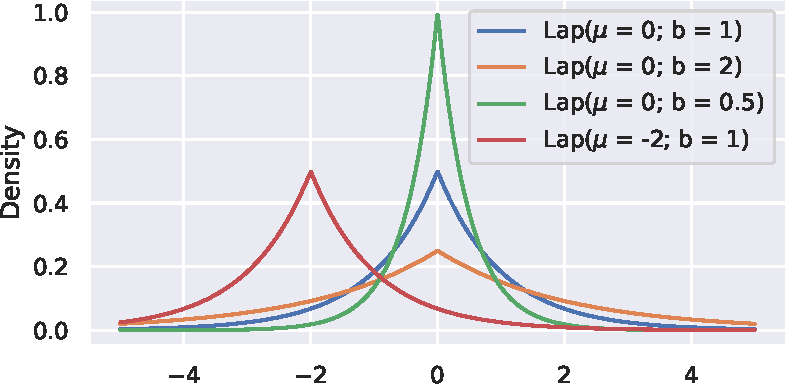
\includegraphics[width=0.8\linewidth]{img/laplace-distributions.pdf}
\caption{Laplace PDF (probability density function)}
\end{figure}
$$
\textrm{Lap}(x; \mu, b) = \frac{1}{2b} \exp \left( - \frac{\abs{x - \mu}}{b}  \right)
$$

%\begin{tikzpicture}[overlay, remember picture]
%\node at (current page.north east)[ref] {
%\fullcite{Voigt.Bussche.2017} \par};
%\end{tikzpicture}
\end{frame}





\begin{frame}{How to choose the parameters?}

Location and scale

-- Location: the true value

-- Scale?

Let's pick $b = 1$ just for lack of better ideas :)

%\begin{tikzpicture}[overlay, remember picture]
%\node at (current page.north east)[ref] {
%\fullcite{Voigt.Bussche.2017} \par};
%\end{tikzpicture}
\end{frame}



\begin{frame}{It's all nice and random, but what does it give us?}

Query: How many persons in the database take illegal drugs?

\begin{table}
\footnotesize
\begin{tabular}{lrrr} \toprule
Name & Hospitalized in year & Age & Illegal drug use \\ \midrule
Alice & 2024 & 32 & yes \\
Bob & 2020 & 21 & no \\
Charlie & 2023 & 45 & no \\
$\ldots$ & & & \\
Xander & 2020 & 31 & yes \\ \bottomrule
\end{tabular}
\caption{Database $D$, including Alice}
\end{table}


Assume that the true answer is 51

%\begin{tikzpicture}[overlay, remember picture]
%\node at (current page.north east)[ref] {
%\fullcite{Voigt.Bussche.2017} \par};
%\end{tikzpicture}
\end{frame}


\begin{frame}{It's all nice and random, but what does it give us?}

What if Alice decided \textbf{not to be part of the data}?

-- She has the right to decide about her privacy, GDPR, etc.

\begin{table}
\footnotesize
\begin{tabular}{lrrr} \toprule
Name & Hospitalized in year & Age & Illegal drug use \\ \midrule
Bob & 2020 & 21 & no \\
Charlie & 2023 & 45 & no \\
$\ldots$ & & & \\
Xander & 2020 & 31 & yes \\ \bottomrule
\end{tabular}
\caption{Database $D'$, \textbf{excluding} Alice}
\end{table}

The true answer to the query would be now 50


%\begin{tikzpicture}[overlay, remember picture]
%\node at (current page.north east)[ref] {
%\fullcite{Voigt.Bussche.2017} \par};
%\end{tikzpicture}
\end{frame}


\begin{frame}{We have two databases: With and without Alice}

Privatize for $D$ (with Alice), true answer is 51
$$
Y \sim \frac{1}{2b} \exp \left( \frac{-\abs{x - 51}}{b} \right) = \frac{1}{2} \exp \left( -\abs{x - 51} \right) 
$$

\begin{figure}
\centering
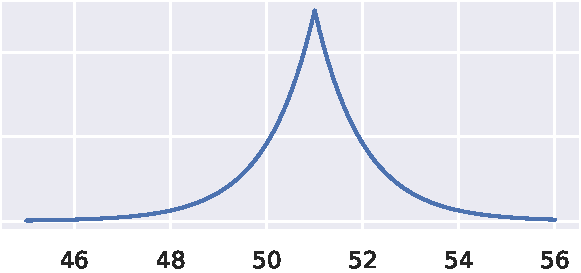
\includegraphics[width=0.7\linewidth]{img/laplace-density1.pdf}
\caption{Laplace density, $\mu = 51, b = 1$}
\end{figure}

%\begin{tikzpicture}[overlay, remember picture]
%\node at (current page.north east)[ref] {
%\fullcite{Voigt.Bussche.2017} \par};
%\end{tikzpicture}
\end{frame}



\begin{frame}{Now without Alice}


Privatize for $D'$ (without Alice), true answer is 50
$$
Y' \sim \frac{1}{2b} \exp \left( \frac{-\abs{x - 50}}{b} \right) = \frac{1}{2} \exp \left( -\abs{x - 50} \right) 
$$


\begin{figure}
\centering
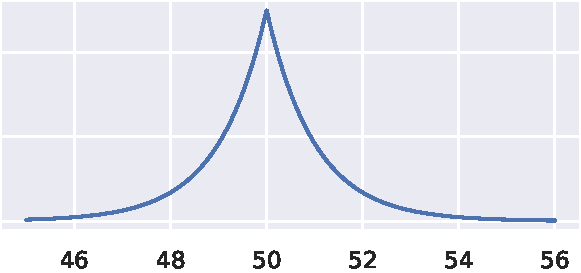
\includegraphics[width=0.7\linewidth]{img/laplace-density2.pdf}
\caption{Laplace density, $\mu = 50, b = 1$}
\end{figure}

%\begin{tikzpicture}[overlay, remember picture]
%\node at (current page.north east)[ref] {
%\fullcite{Voigt.Bussche.2017} \par};
%\end{tikzpicture}
\end{frame}

\begin{frame}{Both variables in one plot}
$
Y \sim  \frac{1}{2} \exp \left( -\abs{x - 51} \right) \qquad
Y' \sim \frac{1}{2} \exp \left( -\abs{x - 50} \right) 
$

\begin{figure}
\centering
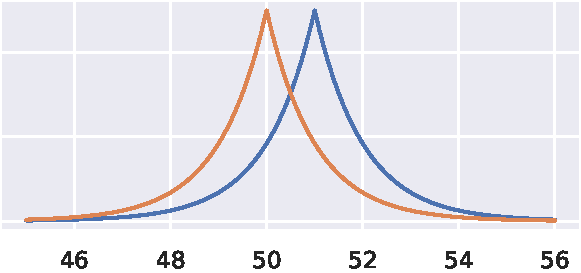
\includegraphics[width=0.6\linewidth]{img/laplace-02.pdf}
\caption{Blue = with Alice, red = without Alice}
\end{figure}

Now observe a particular value $y \in \mathbb{R}$, for example 52

-- Was it sampled from $Y$ or from $Y'$?

%\begin{tikzpicture}[overlay, remember picture]
%\node at (current page.north east)[ref] {
%\fullcite{Voigt.Bussche.2017} \par};
%\end{tikzpicture}
\end{frame}


\begin{frame}{If we observed 52, was it sampled from $Y$ or from $Y'$?}

We cannot really tell!

But we can compare probabilities of this event\footnote{We must compare densities, so our math will not break}

$
\Pr[Y = 52] = \frac{1}{2} \exp \left( -\abs{52 - 51} \right) = 0.5 \exp(-1)
$
$
\Pr[Y' = 52] = \frac{1}{2} \exp \left( -\abs{52 - 50} \right) = 0.5 \exp(-2)
$

How much more likely from $Y$?
$
\frac{\Pr[Y = 52]}{\Pr[Y' = 52]}
= \frac{0.5 \exp(-1)}{0.5 \exp(-2)} = \exp(-1)\exp(2) = \exp(1) = 2.718
$

How much more likely from $Y'$?
$
\frac{\Pr[Y' = 52]}{\Pr[Y = 52]}
= \frac{0.5 \exp(-2)}{0.5 \exp(-1)} = \exp(-1) = 0.367
$

%\begin{tikzpicture}[overlay, remember picture]
%\node at (current page.north east)[ref] {
%\fullcite{Voigt.Bussche.2017} \par};
%\end{tikzpicture}
\end{frame}



\begin{frame}{Both variables in one plot}
$
Y \sim  \frac{1}{2} \exp \left(- \abs{x - 51} \right) \qquad
Y' \sim \frac{1}{2} \exp \left(- \abs{x - 50} \right) 
$

\begin{figure}
\centering
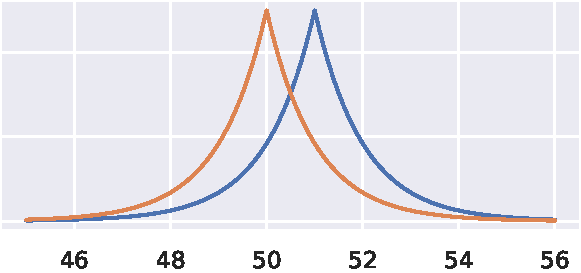
\includegraphics[width=0.6\linewidth]{img/laplace-02.pdf}
\caption{Blue = with Alice, red = without Alice}
\end{figure}

Now observe a particular value $y \in \mathbb{R}$, for example 50

-- Was it sampled from $Y$ or from $Y'$?

%\begin{tikzpicture}[overlay, remember picture]
%\node at (current page.north east)[ref] {
%\fullcite{Voigt.Bussche.2017} \par};
%\end{tikzpicture}
\end{frame}



\begin{frame}{If we observed 50, was it sampled from $Y$ or from $Y'$?}

$
\Pr[Y = 50] = \frac{1}{2} \exp \left(- \abs{50 - 51} \right) = 0.5 \exp(-1)
$
$
\Pr[Y' = 50] = \frac{1}{2} \exp \left(- \abs{50 - 50} \right) = 0.5 \exp(0)
$

How much more likely from $Y$?
$
\frac{\Pr[Y = 50]}{\Pr[Y' = 50]}
= \frac{0.5 \exp(-1)}{0.5 \exp(0)} = \exp(-1) = 0.367
$

How much more likely from $Y'$?
$
\frac{\Pr[Y' = 50]}{\Pr[Y = 50]}
= \frac{0.5 \exp(0)}{0.5 \exp(-1)} = \exp(1) = 2.718
$

It seems like the odds ratio is bounded from above...

%\begin{tikzpicture}[overlay, remember picture]
%\node at (current page.north east)[ref] {
%\fullcite{Voigt.Bussche.2017} \par};
%\end{tikzpicture}
\end{frame}

\begin{frame}{Can we generalize it for any observed $x$?}

\begin{figure}
\centering
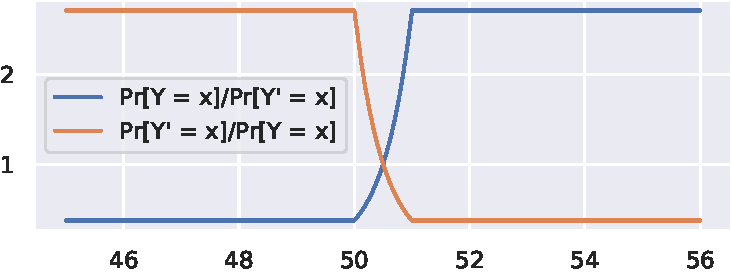
\includegraphics[width=0.8\linewidth]{img/laplace-03.pdf}
\end{figure}

Seems like the maximum we can get is $2.718 = e = \exp(1)$

%\begin{tikzpicture}[overlay, remember picture]
%\node at (current page.north east)[ref] {
%\fullcite{Voigt.Bussche.2017} \par};
%\end{tikzpicture}
\end{frame}


\begin{frame}{Let's try to prove it}

We need triangle inequality for absolute values:\footnote{Homework: Prove it! $x, y \in \mathbb{R}$}
$\abs{x} - \abs{y} \leq \abs{x - y}$

$$
\begin{aligned}
\frac{\Pr[Y = x]}{\Pr[Y' = x]} =
\frac{
\frac{1}{2} \exp \left(- \abs{x - 51} \right)
}{
\frac{1}{2} \exp \left(-\abs{x - 50} \right) 
}
&= \exp ( \abs{x - 50} - \abs{x - 51} ) \\
&\leq \exp ( \abs{(x - 50) - (x - 51)} ) \\
&= \exp ( \abs{x - 50 - x + 51} ) \\
&= \exp ( \abs{1}) = \exp(1) \\
\end{aligned}
$$

\end{frame}


\begin{frame}{Let's try to prove it (part 2)}


$$
\begin{aligned}
\frac{\Pr[Y' = x]}{\Pr[Y = x]} =
\frac{
	\frac{1}{2} \exp \left( - \abs{x - 50} \right)
}{
	\frac{1}{2} \exp \left( - \abs{x - 51} \right) 
}
&= \exp ( \abs{x - 51} - \abs{x - 50} ) \\
&\leq \exp ( \abs{(x - 51) - (x - 50)} ) \\
&= \exp ( \abs{x - 51 - x + 50} ) \\
&= \exp (\abs{-1}) = \exp(1)
\end{aligned}
$$



%\begin{tikzpicture}[overlay, remember picture]
%\node at (current page.north east)[ref] {
%\fullcite{Voigt.Bussche.2017} \par};
%\end{tikzpicture}
\end{frame}


\begin{frame}{What does that mean?}
\begin{figure}
\centering
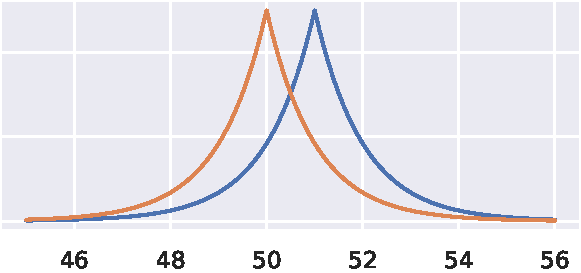
\includegraphics[width=0.4\linewidth]{img/laplace-02.pdf}
\caption{Blue = with Alice, red = without Alice, $Y \sim  \frac{1}{2} \exp \left(- \abs{x - 51} \right) \qquad
Y' \sim \frac{1}{2} \exp \left(- \abs{x - 50} \right)$}
\end{figure}

$
\frac{\Pr[Y = x]}{\Pr[Y' = x]} \leq \exp(1) \qquad
\frac{\Pr[Y' = x]}{\Pr[Y = x]} \leq \exp(1)
$


No matter what value we get after privatizing the counting query -- we can only get some limited "information" about whether it came from $Y$ or $Y'$.



%\begin{tikzpicture}[overlay, remember picture]
%\node at (current page.north east)[ref] {
%\fullcite{Voigt.Bussche.2017} \par};
%\end{tikzpicture}
\end{frame}





\begin{frame}{What if the true answer would be the same for $D$ and $D'$?}

Alice did not take drugs
$
Y \sim  \frac{1}{2} \exp \left(- \abs{x - 50} \right) \qquad
Y' \sim \frac{1}{2} \exp \left(- \abs{x - 50} \right) 
$

\begin{figure}
\centering
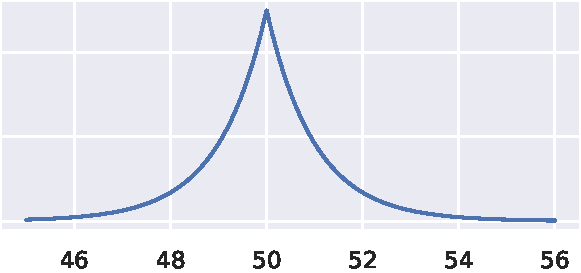
\includegraphics[width=0.4\linewidth]{img/laplace-density2.pdf}
\caption{Both have the same distribution}
\end{figure}

$
\frac{\Pr[Y = x]}{\Pr[Y' = x]} = 1 \leq \exp(1) \qquad
\frac{\Pr[Y' = x]}{\Pr[Y = x]} = 1 \leq \exp(1)
$

So the maximum "loss" only when the presence of Alice changes the query output

%\begin{tikzpicture}[overlay, remember picture]
%\node at (current page.north east)[ref] {
%\fullcite{Voigt.Bussche.2017} \par};
%\end{tikzpicture}
\end{frame}


\begin{frame}{What if the true answer would be 22?}

Alice did not take drugs
$
Y \sim  \frac{1}{2} \exp \left(- \abs{x - 22} \right) \qquad
Y' \sim \frac{1}{2} \exp \left( -\abs{x - 22} \right) 
$

-- bounded by 1 as in the previous slide 

Alice did take drugs

$Y \sim  \frac{1}{2} \exp \left(- \abs{x - 23} \right) \qquad
Y' \sim \frac{1}{2} \exp \left(- \abs{x - 22} \right)$

-- our general proof still holds!
$
\frac{\Pr[Y = x]}{\Pr[Y' = x]} \leq \exp(1) \qquad
\frac{\Pr[Y' = x]}{\Pr[Y = x]} \leq \exp(1)
$

%\begin{tikzpicture}[overlay, remember picture]
%\node at (current page.north east)[ref] {
%\fullcite{Voigt.Bussche.2017} \par};
%\end{tikzpicture}
\end{frame}


\begin{frame}{Summary}

Four counting queries, the maximum difference of the query result is 1 (when a particular person is not in the dataset)

We used scale $b = 1$ for the Laplace distribution, which gives us upper bound on privacy loss

$
\frac{\Pr[Y = x]}{\Pr[Y' = x]} \leq \exp(1) \qquad
\frac{\Pr[Y' = x]}{\Pr[Y = x]} \leq \exp(1)
$

%\begin{tikzpicture}[overlay, remember picture]
%\node at (current page.north east)[ref] {
%\fullcite{Voigt.Bussche.2017} \par};
%\end{tikzpicture}
\end{frame}




\section{Neighboring datasets}

\begin{frame}{Defining neighboring datasets}
	
We saw that the bound was `symmetric'
$$
\frac{\Pr[Y = y]}{\Pr[Y' = y]} \leq \exp(1) \qquad
\frac{\Pr[Y' = y]}{\Pr[Y = y]} \leq \exp(1)
$$
On the left: One entry less in the denominator (= one entry more in the nominator)

On the right: One entry less in the nominator (= one entry more in the denominator)

The bound holds for any two datasets that \textbf{differ in the presence of one entry} (e.g., one row removed, or on row added) $\rightarrow$ \textbf{neighboring datasets}


\end{frame}

\begin{frame}{Neighboring dataset examples (choice of Alice is arbitrary!)}


\begin{table}
	\footnotesize
	\begin{tabular}{lrrr} \toprule
		Name & Hospitalized in year & Age & Illegal drug use \\ \midrule
		Alice & 2024 & 32 & yes \\
		Bob & 2020 & 21 & no \\
		Charlie & 2023 & 45 & no \\ \bottomrule
	\end{tabular}
	\caption{Database 1, including Alice}
\end{table}

\begin{table}
	\footnotesize
	\begin{tabular}{lrrr} \toprule
		Name & Hospitalized in year & Age & Illegal drug use \\ \midrule
		Bob & 2020 & 21 & no \\
		Charlie & 2023 & 45 & no \\ \bottomrule
	\end{tabular}
	\caption{Database 2, excluding Alice}
\end{table}
	
\end{frame}

\begin{frame}{Neighboring dataset examples}

Databases 1 and 2 from the previous slide are \textbf{neighboring} as they differ in presence or absence of a single row

We denote them 1: $D$ and 2: $D'$ \textbf{(an arbitrary choice)}

The neighboring dataset definition allows us to simplify
$$
\frac{\Pr[Y = y]}{\Pr[Y' = y]} \leq \exp(1) \qquad
\frac{\Pr[Y' = y]}{\Pr[Y = y]} \leq \exp(1)
$$
into one inequality (where again $Y$ is a random variable based on $D$ and $Y'$ is a random variable based on $D'$)
$$
\frac{\Pr[Y = y]}{\Pr[Y' = y]} \leq \exp(1)
$$

\end{frame}

\begin{frame}{Restating our bound with neighboring datasets}

Neighboring datasets = presence or absence of a single individual

Our bound $\frac{\Pr[Y = y]}{\Pr[Y' = y]} \leq \exp(1)$ holds for any neighboring datasets (we proved it, but convince yourself again)

So the absence or presence of \textbf{any single individual}
\begin{itemize}
	\item will influence the result of the counting query (but we want to keep this influence small $\rightarrow$ \textbf{utility})
	\item for any `all-mighty' adversary, the likelihood to find out the extra person's `private bit' (e.g., drug use) is upper bounded (the person wants to keep this bound small $\rightarrow$ \textbf{privacy})
\end{itemize}

\end{frame}



\section{Controlling privacy strength}

\begin{frame}{What if 2.718 is not strong enough?}

For $y \sim y_{\mathrm{true}} + \textrm{Lap}(b=1)$

The likelihood for preferring one hypothesis over the other	
$$
\frac{\Pr[Y = y]}{\Pr[Y' = y]} \leq \exp(1) \approx 2.718
$$

What would be the minimum of $\frac{\Pr[Y = y]}{\Pr[Y' = y]}$?

What would be the maximum of $\frac{\Pr[Y = y]}{\Pr[Y' = y]}$?

\pause

$$1 \leq \frac{\Pr[Y = y]}{\Pr[Y' = y]} \leq \infty$$
Why?

	
\end{frame}




\begin{frame}{Playing with the scale parameter $b$}

For $y \sim y_{\mathrm{true}} + \textrm{Lap}(\mu = 0; b=1)$


\begin{figure}
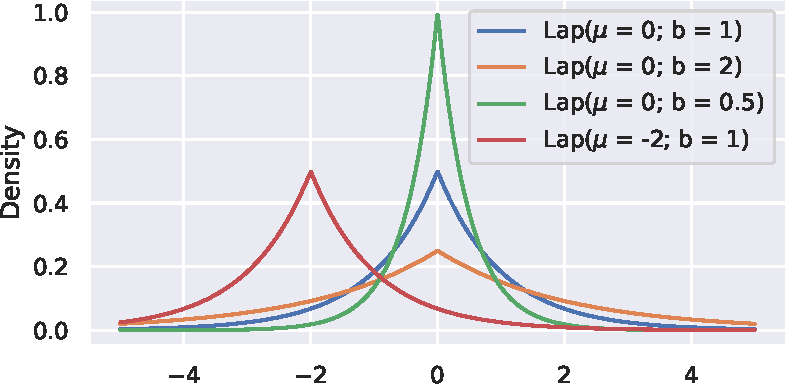
\includegraphics[width=0.6\linewidth]{img/laplace-distributions.pdf}
\caption{Laplace PDF $\textrm{Lap}(x; \mu, b) = \frac{1}{2b} \exp \left( - \frac{\abs{x - \mu}}{b}  \right)$
}
\end{figure}

What to do with the scale for stronger privacy?
	
\end{frame}


\begin{frame}{Intuition: Larger $b$ gives stronger privacy}

\begin{figure}
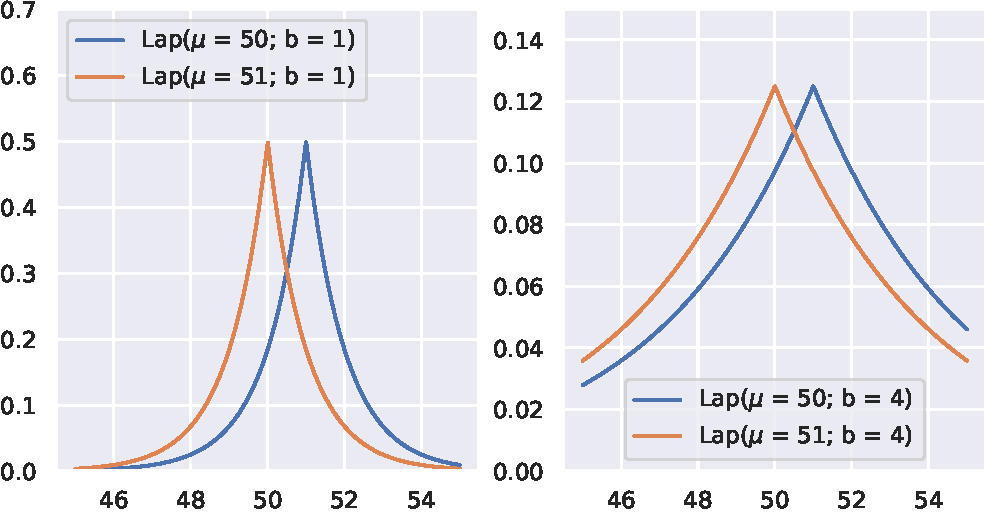
\includegraphics[width=0.9\linewidth]{img/laplace-grid1.pdf}
\caption{Laplace PDF (probability density function)}
\end{figure}
	
\end{frame}


\begin{frame}{How does that relate to the maximum privacy loss?}
Recall: likelihood of any output (x-axis) coming from $D'$ as opposed do $D$ (and vice versa)

\begin{figure}
\centering
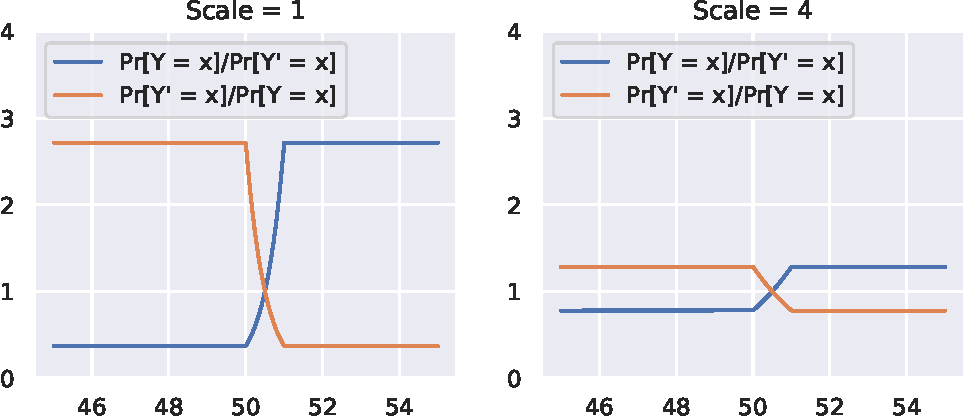
\includegraphics[width=0.8\linewidth]{img/privacy-loss1.pdf}
\caption{Privacy loss for two Laplace distributions for a counting query, varying scale $b$}
\end{figure}

\end{frame}



\begin{frame}{Let's try to formalize our intuition}
\label{slide:proof.reference}

Counting query true value $y= 51$, one person removed $y = 50$
$$
\begin{aligned}
\frac{\Pr[Y = y]}{\Pr[Y' = y]} =
\frac{
\frac{1}{2b} \exp \left(- \frac{1}{b} \abs{y - 51} \right)
}{
\frac{1}{2b} \exp \left(- \frac{1}{b} \abs{y - 50} \right) 
}
&= \exp (\frac{1}{b} ( \abs{y - 50} - \abs{y - 51} ) ) \\
&\leq \exp (\frac{1}{b} \abs{(y - 50) - (y - 51)} ) \\
&= \exp (\frac{1}{b} \abs{y - 50 - y + 51} ) \\
&= \exp (\frac{1}{b} \abs{1}) = \exp(\frac{1}{b}) \\
\end{aligned}
$$
Will be the same for $\frac{\Pr[Y' = y]}{\Pr[Y = y]}$ (prove it! check the appendix)

\end{frame}







\begin{frame}{What have we discovered so far}

Our choice of 50 and 51 was arbitrary, the same proof will hold for any true answers differing by 1

For a \textbf{counting query}, the database curator (\textbf{trusted curator}, trusted holder) protects privacy of each individual by reporting
$$y \sim y_{\mathrm{true}} + \textrm{Lap}(b)$$

This ensures that for \textbf{any two neighboring datasets} the privacy loss is \textbf{bounded}

$$
\frac{\Pr[Y = y]}{\Pr[Y' = y]} \leq \exp(\frac{1}{b})
$$

\end{frame}




\begin{frame}{License and credits}

	\begin{columns}
		\begin{column}{0.7\textwidth}
			Licensed under Creative Commons Attribution-ShareAlike 4.0 International (CC BY-SA 4.0)
		\end{column}
		\begin{column}{0.2\textwidth}
			
\includegraphics[width=0.9\linewidth]{../include/img/cc-by-sa-icon.pdf}
		\end{column}
	\end{columns}
	
	\bigskip
	
	Credits
	
	\begin{scriptsize}
		
		Ivan Habernal
		
		Content from ACL Anthology papers licensed under CC-BY \url{https://www.aclweb.org/anthology}
		
		Partly inspired by lectures from Antti Honkela, Aurélien Bellet, Gautam Kamath
	
	\end{scriptsize}
	
\end{frame}



\end{document}

